%% Main tex for Anomaly Detection paper
%%
%% Author: Rabimba Karanjai (rk45@rice.edu), Jaeho Lee (Jaeho.Lee@rice.edu)
%% Reference: http://www.ctan.org/tex-archive/info/simplified-latex/

%% Revision Control

\documentclass [11pt]{article}
\usepackage[margin=1in]{geometry} %AD... This is the margin line..RK
\usepackage{graphicx}
\usepackage{subcaption}



\title{Anomaly Detection using Behavioral Patterns from SSH Logs\\\medskip Project Proposal}
\author{Rabimba Karanjai (rk45@rice.edu)

\begin{document}
\maketitle
\nocite{*}
\section{Introduction}
\paragraph{}
Our research proposal is to devise the technique of identifying compromised Secure Shell (SSH) accesses from massive log files. We will extract behavior patterns from the log files and apply the statistical method like machine learning to detect anomalies from regular SSH activities. 

Since the intrusion detection model was proposed in 1987 \cite{denning1987intrusion}, there have been a plethora of studies of the intrusion detection using data mining, machine learning, and rule base detection \cite{Gogoi2011}. Also, studies have been conducted using different data sources such as user logs, the sequence of system calls, and packet flow. They propose various intrusion detection techniques both online or offline. However, most of the work have focused on real-time detection so that the approaches require the installation of Intrusion Detection Systems (IDS)
in advance. Also, most of the machine learning approaches assume specific environments so that they are not practical in the general environment, and a few of those work have been applied in the real field \cite{Sommer2010}. Finally, although there are many attacks in SSH servers, there is no research to detect anomalies from the only SSH log file. 

Therefore, our research goal is to devise the practical anomaly detection based on behavioral patterns which are extracted from the SSH server logs. It can be applied in the general environment such as personal machines. This research is important because SSH attacks are common these days \cite{owens2008study} and many people run SSH server on their own personal PC, but they hardly install the IDS or investigate their SSH logs manually to find anomalies. Even in the enterprise machines such as university servers, although they have fancy IDS, they cannot detect malicious users' accesses if they log in without any failure using stolen private keys or passwords. Our goal is also to detect those kinds of accesses. Since our approach extracts the behavioral pattern from the user access logs, we will be able to differentiate accesses to the same account from different users. In this proposal, we will describe our hypothesis and system structure of our final product. Also, we will explain how we will solve challenges in our research. Finally, we shows our literature reviewing result and discuss how we can make the contribution in this field.


\section{Project Proposal}
\subsection{Hypothesis}
\paragraph{} 
In conducting our research, we have two hypothesis. The first one is that it is highly likely that the attacker's behavior deviates from normal user's behavior, which means that the attacker's access pattern to SSH can be differentiated from the normal user's one. For example, the brute-force attack can be easily identified by a bunch of access failures before the successful access, but it is hard for intrusion prevention software like fail2ban to prevent the access of the malicious user who exploits stolen password of a normal user. Nevertheless, malicious user's access pattern will be quite different from the original user. For example, attackers may stay access during the very short time or connect from very strange location. Therefore, if there is enough log history, we can finally find a malicious user's access. If our assumption is correct, when we define behavior patterns well from log files, malicious accesses can be revealed from log files.

The our second hypothesis is that real world SSH log files are complex enough so that we can extract meaningful features and apply statistical method. For example, from the simple connection and disconnection information, we can figure out several information: average accessing time of user, access location pattern, weekly accessing pattern and usual failure frequency. Also, we can get more information from other log events. Therefore, if we analyze real world log file from the different viewpoint, we can extract many meaningful factors and apply them to anomaly detection. Therefore, the start of our work will be to extract meaningful behavioral patterns from raw log files.

\subsection{Design of anomaly detector}
\paragraph{} 
Since we are targeting the practical solution, our final result would be the anomaly detector that is applicable and runs in the general environment. To accomplish this, we need to find the solutions for following challenges.
\begin{itemize}
\item extracting features from the SSH logs as much as we can do correlation analysis
\item deciding which methodology we applied for anomaly detection
\item how to experiment and how to verify our result
\end{itemize}
In this chapter, we will show our design of the system that we came up with to solve those challenges, and explain them in detail. 

\begin{figure}[b!]
\centering
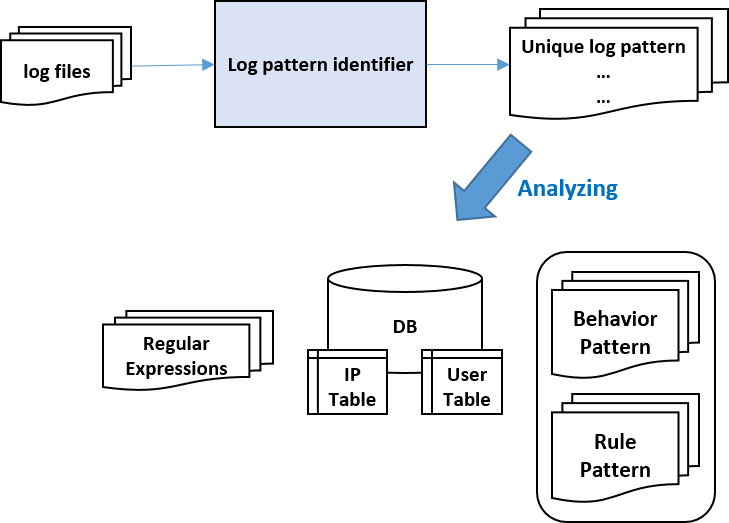
\includegraphics[scale=0.7]{./figures/structure_1.png}
\caption{Identifying log patterns and analyzing}
\label{fig:structure_1}
\end{figure}

\subsubsection{Analyzing logs and extracting patterns}
Our first job is to analyze SSH log files to identify unique log messages and find meaningful log pattern. Figure \ref{fig:structure_1} shows the structure of this phase. Firstly, we will make the log pattern identifier which gets the input of SSH log files and results unique log messages and their frequency. After finding all unique SSH log messages, we will analyze which messages will be meaningful and could be abstracted to high level behavior pattern. After finishing this analysis, we will decide database scheme which includes one level higher abstract information from the raw log files such as user information with connection history and IP information. Also, set of regular expressions that are used later steps and meaningful pattern factors will be extracted. All those information is the key input factors that run our anomaly detector. This analyzing step is repeated literately during whole our development step so that DB schema and patterns are enhanced more and more.
\begin{figure}[b!]
\centering
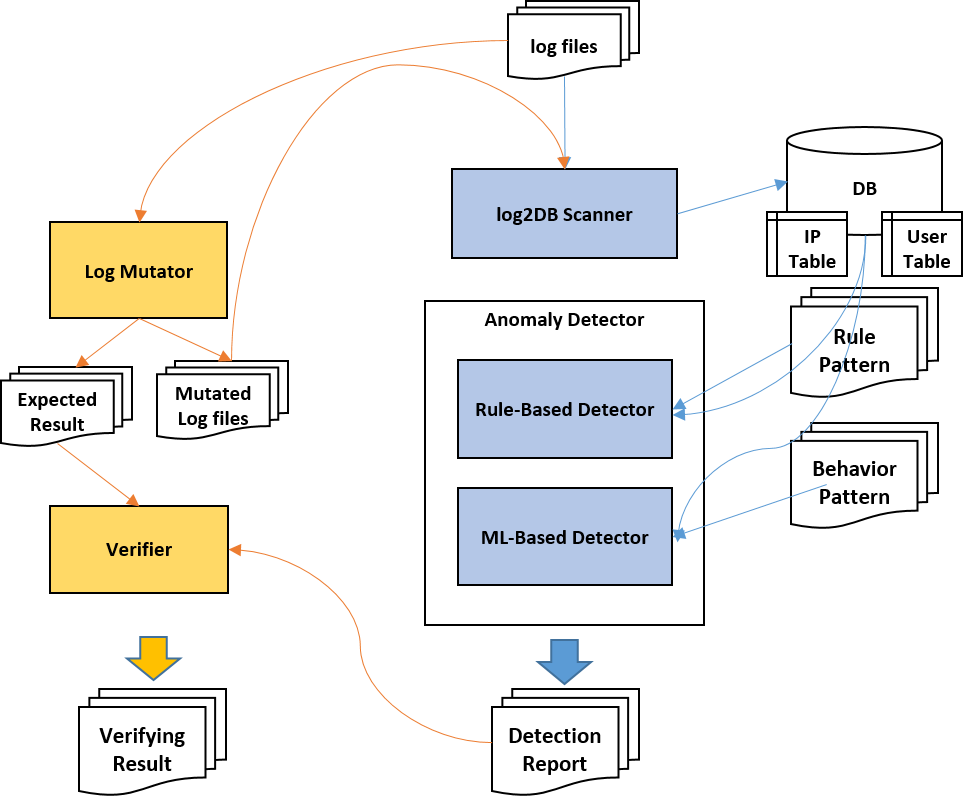
\includegraphics[scale=0.7]{./figures/structure_2.png}
\caption{Structure of anomaly detector and verification modules}
\label{fig:structure_2}
\end{figure}

\subsubsection{Design of anomaly detector}
Figure \ref{fig:structure_2} shows the structure of our anomaly detector we'll implement. The blue rectangular boxes represent anomaly detection modules. Firstly, Log2DB Scanner is the simple parser that fills DB tables from raw log files. This module contains DB-interaction APIs and will be changed every time DB schema is altered. The core of anomaly detection modules is composed of two modules: ML-Based Detector and Rule-Based Detector. ML-Based Detector is our core detector which look through all history DB and define every user's behavior for all given behavior patterns. As soon as defining the behavior of every user, it looks through DB entries further and check if there is any exceptional cases that deviates from the defined patterns. The rule-based detector is the simple rule detector which checks DB tables if there is any violation of the given rule pattern. The rule pattern is the set of predicates such as "Successful login IP should not be in blacklist IP". This rule-based detector will be complementary to the ML-Based Detector. After running those two detectors, detection results are reported.
\subsubsection{Verification Methodology}
One of our challenge is to come up with verification methodology of our system. It is almost impossible to get labeled SSH logs that apparently show which accesses are malicious, but we need labeled date for verification. To deal with this challenge, we came up with the idea that mutates original log files and add some malicious logs randomly. Therefore, we need to implement additional modules. The yellow rectangular boxes in \ref{fig:structure_2} represent verification modules for the anomaly detection system. Log Mutator will mutate the original logs and output a mutated log file and the expected result. Then, the anomaly detector will run with the mutated log file. The verification step will be done by the verifier which compares the detection report from the mutated log and the expected result generated by Log Mutator. If the verification result is not successful, we will look through result, and improve other system by enhancing the detector algorithm and updating DB tables and patterns. This iteration will be repeated until our system will show excellent verification result.

\section{Timeline}

We have decided to divide the project into a few separate pieces. 
\begin{itemize}
\item March 16: Implement log pattern identifier and identify meaningful log pattern manually. 
\item March 23: Design DB schema and implement DB related implementation.
\item March 30: Implement log2DB scanner that parses logs and extracts pattern properties
\subitem We will come up with a way to artificially generate ssh log files with labeled data
\subitem We will use this data to run our machine learning models on and compare our results
\item April 6: Implement anomaly detector
\item April 13: Implement anomaly detector
\item April 22: Implement verifiers and do experiment
\item April 30: Final presentation

\end{itemize}


\subsection{Resources}

We plan to use our artificially generated SSH logs to identify and see if the model can catch anomalous behaviors. Then we plan to use ssh logs from two public servers of Mozilla Corporation to see if our hypothesis holds true for production deployed server logs.

We also plan to utilize some of the rule sets we will find in fail2ban, denyhost, sshguard to understand more about the performance impact and false positives our model may produce. For machine learning we plan to utilize weka to run the algorithms and also python scikit toolkit.

We plan to divide the work in different sections. We both will work on making the pipeline since it needs knowledge about how log files work. Then we plan to divide the work based on modules. We each will handle a different part of the module and manage ownership of it.



\section{Review of the works}
\paragraph{} 

we reviewed papers in three categories: anomaly detection, SSH attack and defense, and effective log analysis. Firstly, anomaly detection has been an active research field for a long time. This is to solve the problem of finding patterns in data that do not conform to expected behavior \cite{chandola2009anomaly}. One of the famous application of anomaly detection is intrusion detection. Most research efforts have addressed the problem of how to improve the performance of IDS by reducing the false alarm rate, increasing coverage of attack types, and boosting the detection rate. To accomplish this, many kinds of research in this area exploit statistical approach or machine learning technique such as neural networks, support vector machines (SVM) and decision trees.    

Secondly, among the growing threats of hacking, SSH attacks are a major area of concern for security people because of its danger associated with a successful compromise \cite{hellemons2012sshcure}. Therefore, there have been studies that identify the threats of SSH attack and improve its security weakness. 

Finally, we reviewed papers which provide the way of detecting anomalies based on user or system log files and helping log analysis easier. We tried to find the effective way of analyzing SSH log files. However, there is no research on this specific topic, but some studies have eased the difficulty of analyzing system logs. 

\subsection{Survey papers for anomaly detection}
In the work \cite{denning1987intrusion}, the intrusion detection model was proposed first. This research described several statistical methods such as threshold measure, mean and standard deviation. Also, the work introduced six main components: subjects, objects, audit records, profiles, anomaly records and activity rules. Data mining and machine learning for classification were also proposed which has influenced intrusion detection studies later on. Since this research, a variety of research have been conducted in finding anomaly detection, and there has been also many survey papers.

Varun Chandola, Arindam Banerjee and Vipin Kumar provided two comprehensive overviews of existing anomaly detection methods in 2007 \cite{chandola2007} and 2009 \cite{chandola2009anomaly}. They classified anomalies into three categories: point anomaly, a contextual anomaly, and a collective anomaly. Also, they classified intrusion detection techniques into two categories (network intrusion detection and host-based intrusion detection), then provided a structured and broad overview of existing studies as the following. 
\begin{itemize}
\item Statistical Profiling using Histograms (22 papers)
\item Parametric Statistical Modeling and Non-Parametric Statistical Modeling (3 papers)
\item Bayesian Networks (4 papers)
\item Neural Networks (8 papers)
\item Support Vector Machines (3 papers)
\item Rule-Based Systems (7 papers)
\item Clustering Based (4 papers)
\item Nearest Neighbor-Based (2 papers)
\item Spectral (4 papers)
\item Information Theoretic (2 papers)
\end{itemize}

Prasanta Gogoi et al \cite{Gogoi2011} did a survey of outlier detection
methods in network anomaly identification. They first formalize a definition of outliers and then go over different distance and density based methods for outlier detection.

V Jyothsna et al \cite{Jyothsna2011} divided the field of anomaly detection into two groups, based on signature and anomaly. They defined approach and methods, and categorized papers to various models: statistical based, operational or threshold metric model, statistical moments or mean and standard deviation model, uni-variate model, multivariate model, time series model, outlier detection model, or user intention based.

F\'{a}bio Bezerra and Jacques Wainer \cite{Bezerra2013} proposed four algorithms for detecting anomalies in logs of the process-aware system. They use control flow approach to detect anomalies. They have defined anomalies with the help of some intuitions, like the frequency of an individual execution of the event, the noise, and the mined model. They evaluate the performance of their threshold, iterative and sampling algorithms on a set of artificial logs they create and also later on over real logs.

\subsection{Machine Learning for anomaly detection}
The most vibrant research trend in anomaly detection is to apply machine learning technique to identify anomalies. There are many proposed techniques that could identify attacks: Artificial Neural Network and RIPPER for analyzing the sequence of system calls, k-nearest neighbor for the frequency of system calls, Support Vector Machine for TCP/IP data stream and user logs.

\subsubsection*{Artificial neural network and support vector machine}
Wun-Hwa Chen et al \cite{chen2005application} discussed Artificial Neural Network and Support Vector Machine techniques for classifying data for anomaly detection by comparison. They used Artificial Neural Network trained with back-propagation algorithm to predict intrusion. Also, they used KDD dataset to test their approach. To parse the system calls, they took a frequency-based encoding method by aggregating system call information for the entire execution of a process to characterize program behavior. Each process is first represented as the vector, where each entry represents the occurrence of a specific system call during execution. They prepared a frequency distribution of system calls for normal and abnormal processes. Finally, they experimented with SVM and term frequency–inverse document frequency (tf-idf) encoding methods and came to the conclusion that SVM performance was better than Artificial Neural Network also tf-idf to be better than simple frequency-based methods.

\subsubsection*{K-nearest neighbor}
Ming-Yang Su \cite{DBLP:journals/eswa/Su11} proposed a method which can detect large-scale
attacks, such as DoS attacks, in real time by weighted k-nearest neighbor classifiers (KNN). The key factor for designing an anomaly based NIDS is to select significant features for making the decision. They proposed a Genetic Algorithm combined with KNN for feature
selection. They also used the KDD Cup 99 data-set for experimentation. All initial 35
features in the training phase were weighted, and the top ones were selected to
implement network intrusion detection system for testing. Many Denial of Service (DoS) attacks were applied to evaluate the performance of the system.

\subsubsection*{Hidden Markov model}
In the work \cite{sperotto2012autonomic}, they propose an autonomic way for tuning the SSH parameters of anomaly-based intrusion detection systems. They highlighted more in tuning the parameters to enhance the performance of anomaly detection. To optimize procedure, they used Hidden Markov Model.

\subsubsection*{Bayesian algorithm}
Dewan Md. Farid and Mohammad Zahidur Rahman \cite{dewan2011} presented the
approach to the alert classification to reduce the false positive in Intrusion detection
using Self-Adaptive Bayesian Algorithm (ISABA). The proposed approach applied to
the security domain of anomaly based network intrusion detection, which correctly
classifies different types of attacks of KDD99 benchmark dataset with high
classification rates in short response time and reduces false positive using limited
computational resources. It analyzes the large volume of network data and considers
the complex properties of attack behaviors to improve the performance of detection
speed and detection accuracy.

\subsubsection*{General}
Also, there are many studies using data mining and attempts to increase the speed of classification in anomaly detection. Firstly, Mansour Sheikhan and Amir Ali Sha'bani \cite{sheikhan2009fast} developed two mechanisms to achieve a fast intrusion detection system. In the first one, the training speed of neural attack classifier is improved by using output weight optimization hidden
weight optimization (OWO-HWO) training algorithm, and in the other one, a feature relevance analysis is performed to decrease the number of input features and size of the neural classifier.

Mohammadjafar Esmaeili and Arwa Almadan \cite{Esmaeili2011} proposed using a sliding window approach in combination with a signature based approach in order to detect anomalies by comparing previously clustered data.

In the work \cite{Kind2009}, they proposed feature-based anomaly detection using histogram-based traffic information. They defined features for TCP network flow such as source IP, destination IP, port numbers and so on. Then, based on these features, they cluster TCP streams, construct histogram models and find anomalies.

\subsection{Fuzzy logic}
In the paper \cite{shanmugavadivu2011network}, the authors proposed a fuzzy logic-based system for effectively identifying the intrusion activities within a network. The system supposedly is able to detect an intrusion behavior of the networks since the rule base contains a better set of rules. 
The authors have used an automated strategy for the generation of fuzzy rules, which
are obtained from the definite rules using frequent items. The experiments and evaluations of the proposed intrusion detection system are performed with the KDD Cup 99 intrusion detection dataset.

\subsection{SSH Attack}
Since the advent of SSH, people have accessed remote machines without the concern of threat like snipping our communication. However, SSH attacks have become a major security concern because of its danger associated with a successful compromise\cite{hellemons2012sshcure}. Therefore, there have been many studies related to SSH attacks and defenses. 

In the works \cite{owens2008study,ramsbrock2007profiling,seifert2006analyzing}, they showed the threat of SSH attacks and how they are common nowadays. Also, there has been many efforts to enhance SSH security. the one of major research is to detect SSH attacks in advance. There are two types of studies. In \cite{hellemons2012sshcure}, they propose effective detection of SSH attacks by installing modified SSH client called SSHCure. Also, in \cite{hofstede2014ssh}, they provide to find compromise detection by analyzing network flow. The both of them are to aim to find SSH attack in real time.

\subsection{Analysis based on log file}
We reviewed papers which provide the way of detecting anomaly based on log files and helping log analysis easier. 

Firstly, Adrian Frei and Marc Rennhard \cite{Frei2008} presented an approach for detecting and visualizing
anomalies in a log file using word count to create a single predictor attribute which they use to create a histogram for each log line every hour. Then they applied a bespoke statistical measure as their anomaly detection method based on the standard deviation of each individual bin’s values compared to the same bins over the current day or same slot on a previous week for comparison.

Advances and Challenges in Log Analysis: 
In this journal \cite{Oliner2012}, the authors talk about some of the most common application of log analysis, problems in using statistical methods in log analysis and some methods people use to analyze logs. They argue that the effectiveness of log analysis will depend upon the type of attacks we are trying to detect with the type of logs we have. Citing the example of ssh logs and the data we have within them, they have explained that this kind of logs give us limited data in terms of login, logout time, failed login attempts, IP association with the user. From this information, it is possible to analyze user behaviors but not reliable considering events like a vacation. They also argue that though we can use statistical anomaly detection to mine from anomalies, they do not provide any actionable insight. They have observed that to make detection and prediction easier a lot of recent work aims to modify the instrumentation so that logs have more helpful data for specific kind of analysis. 

In the work \cite{Taerat2011}, they propose a method which tackles the 
issues of clustering of extremely large log files and compares the performance of their
solution against other common methods. From this work, additional predictor attributes can be identified and tested. This work can be combined with HMAT by \cite{Frei2008} to build a new approach to anomaly detection.

Wei Xu \cite{Xu2009} proposes a method in their paper which first creates composite features by analyzing console logs and then use these features in machine learning to detect operational anomalies in the log. Their method can be summarized as a four step process. In the first step, they parse the log file and static code analysis is employed to generate an abstract syntax tree (AST) of the logger class of the logger. AST gives all method calls on objects of the classes with filename and number of the call. By enumerating toString call in classes they are able to deduce the type of variables which are used in logging. Once this is produced all possible log message template strings are collected from the source code and match these templates to each log message to recover its structure, effectively building a schema for the console logs. In the second step, state ratio and message count vectors are created as feature vectors. The state ratio vector is created exploiting a time window between which group of state variables is represented. The actual number does not matter but the ratio between state variable changes matter. Each dimension of the vector corresponds to a distinct state variable value, and the value of the dimension is how many times this state value appears in the time window. The message count vector are based on identifiers. For a specific identifier, all the actions related to that identifier is grouped to create a message count vector. Each vector dimension corresponds to a different message type, and the value of the dimension tells how many messages of that type appear in the message group similar to a bag of words if we consider the message groups as `document'.In the third step, Principal Component Analysis is used for anomaly detection. PCA initially is employed to separate out repeating patterns in feature vectors, thereby making abnormal message patterns easier to detect. Once the `normal' behaviors are pruned anomalies are computed by computing the farthest away events from the sub-space. To further improve the processing, Term Frequency-Inverse Document Frequency (TF-IDF) is used in the feature matrix. Intuitively, multiplying the original count with the IDF reduces the weight of common message types that appear in most groups, which are less likely to indicate problems. This is not applied to state-ratio vectors. These methods are used in logs collected from HDFS file system and Darkstar game server console logs. They were able to detect performance problems in the system with the high load using the state vectors.They also could mark the recovery period as anomaly using the message count vector. Similarly for HDFS they were able to detect anomalies due to transient workload imbalance. In the last step, a decision tree was created to give more insight to the PCA. The PCA results were used as class labels and RapidMiner was used to generate the decision tree.

Finally, in work \cite{lou2010mining,rouillard2004real}, the authors provide the effective way of log file analysis and the technique of correlating events in the log. Also, using these techniques, they suggest the effective way of detecting system problems without huge manual labor.


\section{Experiments}
\subsection{Principal Component Analysis}

In the context of detecting anomalies in log files, PCA can help to filter frequently repeating patterns in the data which makes it easier to detect anomalies. Basically, PCA finds dimensions that have the largest variances and sorts the dimensions in such a way that the first dimension contains the largest portion of the total variance and the last dimension the lowest portion. We try to see the variance of the data we have by trying Principal Component Analysis on it. The features we use for this are date, log in time, user, IP address logged from. The log in time is always increasing and will be mostly bulked into similar groups if most people try to log in at the same time. We expected to get the variance from the data to detect outliers\cite{PCA} in our data. We ran PCA on the whole data set with 284 unique users. The result we got pointed us the outliers in our data point which are probable anomalies in the dataset[Figure 3.a].
\begin{figure}[h]
\centering
%\begin{minipage}{.3\textwidth}
%\centering
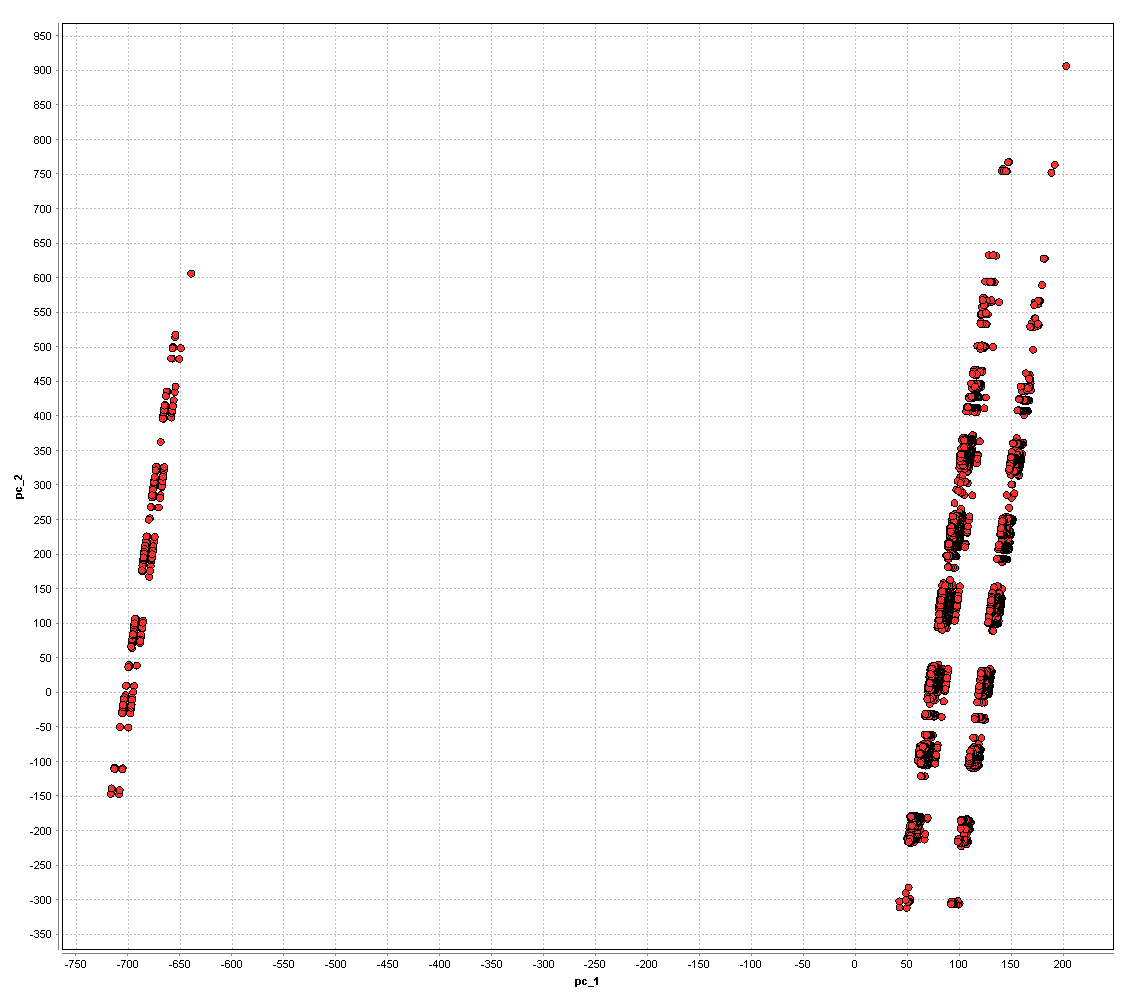
\includegraphics[totalheight=0.25\textheight]{./figures/PCA-PAper.png}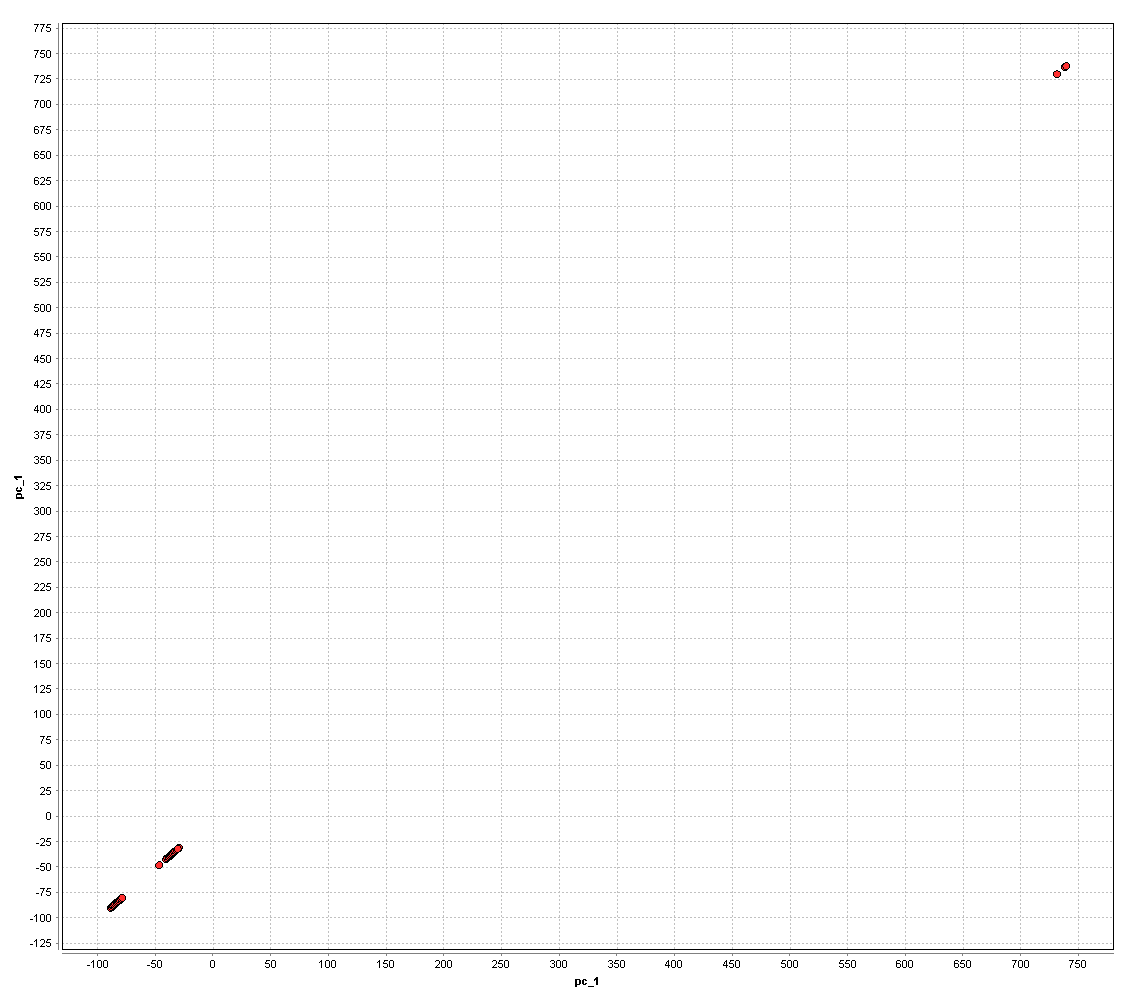
\includegraphics[totalheight=0.25\textheight]{./figures/PCA_User1.png}
\caption{(a) and (b)}
%\end{minipage}
% \begin{minipage}{.3\textwidth}
% \centering

% \end{minipage}
\end{figure}



However this does not give us much insight into what is wrong. We can select the outlier and point it out to the anomalous log but it doesn't tell us why it is an anomaly. Also we realized that in the log data we have, the user distribution is not even. Some users have a lot of activity and some very few. So a user specific activity profiling may give us much better outlier. Which we tried on a specific user with highest number of activity and got the following activity[Figure3.b]

\subsection{K-Means Clustering}
The k-means clustering algorithm is commonly used for cluster analysis since it is fast and rather easy to implement. The algorithm tries to find groups of data instances with similar size and low variance. Given a number k and an initial set of cluster centroids, standard k-means first assigns each data instance in the set to the nearest.centroid using the euclidean metric. It then calculates a new centroid for each cluster by computing the means between all data points in the cluster. These two steps are repeated recursively until the centroid for all clusters does not change anymore. For our case\cite{KMean} we take the feature sets of Start Time, End Time, User, Logged in Duration as our features and try to map out outliers [Figure 4].
\begin{figure}
\centering
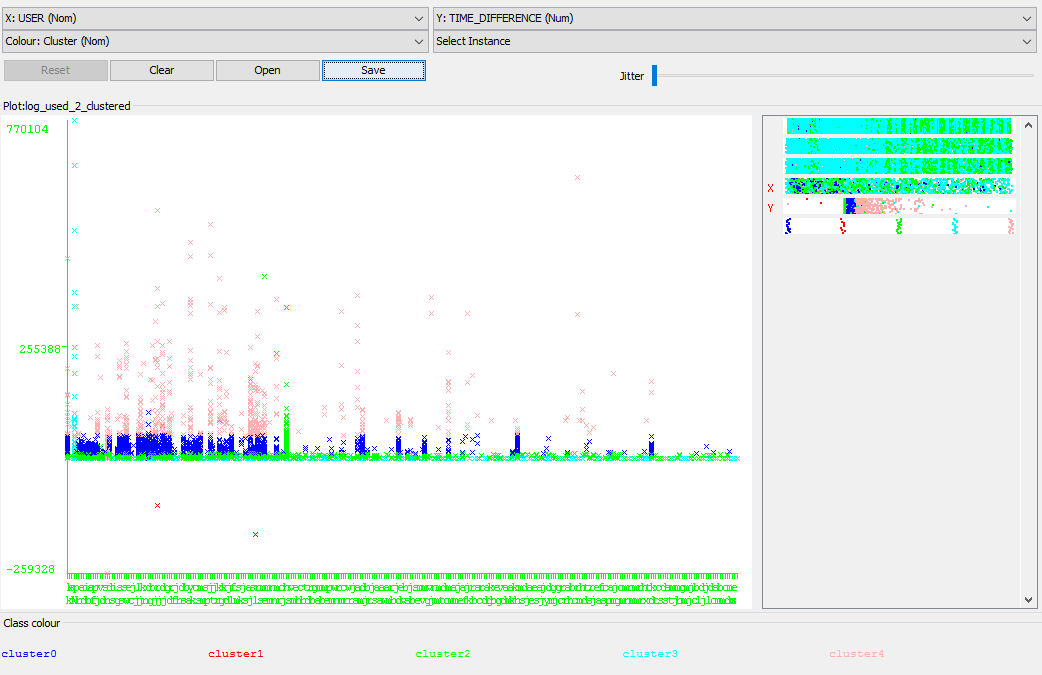
\includegraphics[totalheight=0.25\textheight]{./figures/userVSdur.PNG}
\caption{}
\end{figure}
In this case the X axis denotes each user and the Y axis denotes the duration of his activity. We can see that from this graph there are two points in the log which have negative duration. Which is not possible. That helped us find erroneous log entries and entries which our parser ahd parsed incorrectly. we also got different types of graphs from it to see what other data we can get. This encouraged us to experiment more with this approach with another set of vectors with user,time duration and IP logged in from.

\section{Future Work and Timeline}

We plan to experiment more with the above approaches and come up with more feature vectors which should give us more interesting data points. However along with those we want to study the following methods with our data to see what results they produce.

\subsection{Time Series Clustering}

Since our log data is basically a time series of each users behavior. We can cluster their behavior based on a time series. Since we don't have any other metadata available, the assumption here is their interesting activities are representative of their logged in time and how long they have been logged in, and the corresponding pattern that will emerge. Once we have it we can use KDD Cup SSH dataset to train a classifier and run it on our data to verify. Right now we are trying to process our data to run some tests for this method.

\subsection{Frequent Itemset Mining}
We plan to mine for patterns among the data and cluster them. This method will find similar kind of usage patterns among the log, based on the log activities we have along with user and IP consideration. This will cluster similar time of logs and the smaller or outliers will be our anomaly. We have tried to run some test with this method with different support vectors and though it does cluster different log types. It seems the best result will be if we first bin our log files based on user activities and then run it on those bins. SO each bin will behave as a separate item and it will cluster the similar bins together.Outliers will be our anomaly. We are now in the process of separating data into chunks.

\section{Discussion and Challenges}

While reviewing papers, we could notice two interesting points. Firstly, most of the studies are done based on machine learning techniques, but there are two limitations using machine learning in the area. Firstly, even though there are a lot of anomaly research using machine learning, they have rarely been used in the practical field \cite{Sommer2010}. The authors of the work \cite{Sommer2010} claim that machine learning techniques seem to effective in anomaly detection, but it is very hard to apply to the real fields. This is because many kinds of research work in its limited environment and have very high costs of classification errors. Therefore, there is a certain semantic gap between research results and their operational interpretation.

In addition to this problem, we found many studies that we reviewed used KDD Cup 1999 Data \cite{hettich1999uci}  in the experiment to evaluate machine learning schemes. In practice, this dataset is decade old and has many criticisms \cite{mahoney2003analysis,mchugh2000testing} for current research. Because of those reasons, many applications of anomaly detection using machine learning are not applicable in the real field. 

During the review process, we tried to find the research that has the same goal as ours, but we couldn't find one that has the same goal with the same limitation. We suppose that this is because there are two challenges in our research that lead people not to conduct this research. Firstly, SSH log file seems to be too simple to use machine learning or cutting-edge concepts. Therefore, getting the desirable result using only one type of log file seems to be difficult and it doesn't seem interesting. Secondly, it is hard to experiment to test our result after implementing because it is hard to get labeled data. 

Considering those observations and situations, it will be meaningful if we could find the reasonable way of experiment and make the practical solution based on SSH log. 

We want to test our approach that a successful anomaly detection should be possible by applying machine learning methods to learn behavior from logs. Using these insight we want to test whether we can use machine learning to come up with a system that can analyze and detect anomalies in server SSH logs with fewer or comparable false positives than present state of the art rule based anomaly detection systems. 

\bibliographystyle{IEEEannot}
\bibliography{annot}
\end{document}